\documentclass{techrep}
\usepackage[T1]{fontenc}
\usepackage{amsmath, bm}
\usepackage{fancyhdr}
\usepackage{array}
\usepackage{stmaryrd}
\usepackage{graphicx}
\usepackage{gensymb}
\usepackage{vaucanson-g}
\usepackage{amsfonts}
\usepackage{float}
\usepackage{verbatim}
\usepackage{makeidx}
\usepackage{lmodern}
\usepackage{amsmath}
\usepackage{amsthm}
\usepackage{amsfonts}
\usepackage{tikz}
\usepackage{listings}

\usetikzlibrary{automata,positioning}
\title{SpeakerID - Spherical Discriminant Analysis}
\author{Victor Lenoir} \revision$LastChangedRevision: 2340 $
\date{January 2013} \email{lenoir@lrde.epita.fr}

\definecolor{dkgreen}{rgb}{0,0.6,0}
\definecolor{gray}{rgb}{0.5,0.5,0.5}
\definecolor{mauve}{rgb}{0.58,0,0.82}
\definecolor{colKeys}{rgb}{0,0,1}
\definecolor{colIdentifier}{rgb}{0,0,0}
\definecolor{colComments}{rgb}{0,0.5,1}
\definecolor{colString}{rgb}{0.6,0.1,0.1}

\lstset{
  language=Python,
  basicstyle=\footnotesize,
  numbers=left,
  numberstyle=\tiny\color{gray},
  stepnumber=2,
  numbersep=5pt,
  backgroundcolor=\color{white},
  showspaces=false,
  showstringspaces=false,
  showtabs=false,
  frame=single,
  rulecolor=\color{black},
  tabsize=2,
  captionpos=b,
  breaklines=true,
  breakatwhitespace=false,
  title=\lstname,
  keywordstyle=\color{blue},
  commentstyle=\color{dkgreen},
  stringstyle=\color{mauve},
  escapeinside={\%*}{*)},
  morekeywords={*,...}
}

\lstset{
  float=hbp,
  basicstyle=\ttfamily\small,
  identifierstyle=\color{colIdentifier},
  keywordstyle=\color{colKeys},
  stringstyle=\color{colString},
  commentstyle=\color{colComments},
  frameround=tttt,
  extendedchars=true,
  showspaces=false,
  showstringspaces=false,
  numbers=left,
  numberstyle=\tiny,
  breaklines=true,
  breakautoindent=true,
  captionpos=b,
}

\summary{The purpose of a speaker verification system is to check
  whether a hypothesized speaker is really the author of a speech
  utterance. Currently, the best performances are performed using a
  mapping of each speaker utterance to a low dimensional vector called
  I-vector. The speaker verification score is computed thanks to a
  cosine distance between these two vectors representing both a
  speaker.


  In this paper, we describe a dimensionality reduction technique
  called Spherical Discriminant Analysis (SDA).  The goals of this
  projection are to maximize the cosine distance between different
  speaker's utterances and minimize the cosine distance between same
  speaker's utterances; it has been shown that SDA subspace, which is
  more suitable for the cosine distance than Linear Discriminant
  Analysis (LDA), yields superior performance in face recognition
  task. We will compare the SDA subspace performance with the standard
  LDA approach.}

\frenchsummary{La r\^ole de la v\'erification de locuteur est de
  v\'erifier l'identit\'e pr\'esum\'ee d'un segment de parole. Actuellement,
  les meilleures performances sont obtenus par un mapping de chaque
  segment de parole d'un locuteur vers un vecteur appel\'e I-vector. Le
  score de la v\'erification de locuteur est calcul\'e par une distance
  cosine entre ces deux vecteurs repr\'esentant chacun un locuteur.

  Ce rapport d\'ecrit une technique de r\'eduction de dimension
  appel\'ee Spherical Discriminant Analysis (SDA). Les objectifs de
  cette projection sont de maximiser la distance cosinus entre deux
  locuteurs diff\'erents et de minimiser la distance cosinus entre
  deux m\^eme locuteurs; il a \'et\'e montr\'e que le sous-espace de
  la SDA, qui est plus appropri\'e pour la distance cosinus que la
  Linear Discriminant Analysis (LDA), obtient de meilleur performance
  en reconnaissance faciale. Nous allons comparer les performances
  obtenues par la SDA avec celles obtenues par la LDA.}

\keywords{speaker verification, dimensionality reduction, subspaces,
  ivector, cosine distance}

\begin{document}

\section*{Copying this document}
Copyright \copyright{} 2012 LRDE.

Permission is granted to copy, distribute and/or modify this document
under the terms of the GNU Free Documentation License, Version 1.2 or
any later version published by the Free Software Foundation; with the
Invariant Sections being just ``Copying this document'', no
Front-Cover Texts, and no Back-Cover Texts.

A copy of the license is provided in the file COPYING.DOC.

\tableofcontents

\newpage

\chapter*{Introduction}
%TODO: Une introduction avec le contexte général de votre travail, une
%description des problèmes auxquels vous voulez répondre et comment
%vous y répondez.  L’introduction doit capturer le lecteur et lui
%donner envie de lire la suite. Elle doit donner assez d’informations
%pour que celui-ci puisse comprendre l’intérêt de votre travail et la
%portée de vos résultats.  Plan
\chapter{Context: Speaker verification system}

Nowadays, in a lot of secure applications, people have to prove their
own identity to go into a critical system. Most of these applications
are based on password authentications as in bank cash points or in the
access of some protected buildings. However, in such systems, a robber
can easily find the password and use it to gain access to the critical
area. For this reason, more and more authentication systems are based
on bio-metrical features like fingerprints, iris or voice which present
more inviolable features. Indeed, the study of these bio-metrical
features is an expanding research field. Furthermore, it is known that
fingerprints have been used extensively in criminal investigations for
a long time. Today, voice recognition systems are beginning to have a
legal status in some countries as a proof to authenticate a speaker on
a tape recording.  In this report, we consider the problem of voice
authentication, generally called the speaker verification
problem. More precisely, we focus on the text-independent speaker
verification, i.e. we do not consider the uttered text.\\\\ In our
speaker verification task, speakers are first modeled from enrollment
data coming from phone recordings. During the verification task, these
models enable to check whether a segment of speech is uttered by a
hypothesized speaker. For a few years, the community has been more and
more interested in resolving this verification problem even if the
enrollment conditions are different during the training step and the
testing step.

\section{Speaker verification system}

A speaker verification system is a complex system. In this part I will
try to quickly describe each part of a speaker verification system to
have a general view.

\tikzstyle{cont}=[shape=rectangle,minimum
  size=1.0cm,draw=blue!70,fill=blue!30,font=\small]

\tikzstyle{contred}=[shape=rectangle,minimum
  size=1.0cm,draw=red!70,fill=red!30,font=\small]

\begin{figure}[H]
  \begin{center}
    \begin{tikzpicture}[scale=0.8,font=\scriptsize]
      \node[cont,initial above] (s1) at (0,0) {Audio signal};
      \node[cont] (s2) at (0,-2) {Audio features}
      edge [<-] node[left] {Features extraction} (s1);
      \node[cont] (s3) at (0,-4) {Speaker features}
      edge [<-] node[left] {Voice Activity Detection/Speaker diarization} (s2);
      \node[cont] (s4) at (0,-6) {Speaker model}
      edge [<-] node[left] {Modeling} (s3);
      \node[cont] (s5) at (0,-8) {Low-dimensional speaker model}
      edge [<-] node[auto] {\textcolor{red}{Dimension reduction}} (s4);
      \node[cont] (s6) at (5,-10) {Low-dimensional speaker model};
      \node[cont] (s7) at (0,-10) {Score}
      edge [<-] node[auto] {Scoring} (s5)
      edge [<-] node[auto] {Scoring} (s6);
      \node[cont] (s8) at (0,-12) {Decision}
      edge [<-] node[auto] {Threshold} (s7);
    \end{tikzpicture}
  \end{center}
  \caption{Flowchart of a speaker verification system.}
  \label{flowchart_svs}
\end{figure}

Let's have a closer look to each part of this system.

\subsection{Features extraction}

The features extraction consists in extract, from a raw signal or a
preprocessed signal, features that represent more accurately the
human speech.

Raw speech signals are difficult to process since the information held
is very dense and for the most part not useful when it comes to speech
recognition or speaker verification. In order to focus on the
important information, it is common to proceed with feature
extraction.  Feature extraction is the process of collecting a set of
coefficients that represent as accurately as possible phonetic events,
thus changing the sound representation to a more suitable one for
further processing.

\subsection{Voice activity detection/Speaker diarization}

\paragraph{Voice activity detection} Voice activity detection is a technique used to detect human speech from a signal.
The idea is to separate speech segment from silence and noise.

\paragraph{Speaker diarization} Speaker diarization is the process of partitioning a raw signal into segments assigned to different speakers. This problem consists in determining the number of speakers in a given signal
and in partitioning this signal into segments. It's a mandatory step for speaker verification systems.

This part of the process is useful because the noise and silence corrupts the speaker model.

\subsection{Modeling}

Modeling resides in finding a unique representation (a model) of a
speaker from the speaker features.  For example, a naive model would be
to compute the mean of the speaker features (which is equivalent to a
Gaussian model). Then, the model would be a vector of the dimension of
the features.

\subsection{Dimension reduction}

The goal of the dimension reduction is to find a model subspace which yields
superior classification performance than the original model space.

\subsection{Scoring}

The scoring is the comparison of two speaker models. The scoring
results in a score of likeness of the models.

\subsection{Threshold}

The final goal of a well-tuned speaker verification system is to make a decision
on whether the given sound data has been indeed produced by the person who proclaims
to be the speaker.
To take a final decision, we just have to threshold the computed score.

%BONUS: NAIVE EXAMPLE OF SPEAKER RECO? AWESOME!

\section{Dimension reduction}

In this paper, we are only interested in the dimension reduction
process. The idea is to find a subspace which yields superior
classification performance than the original space. One of the most
known dimension reduction technique is the Linear Discriminant
Analysis (LDA).

The goal of the LDA is to maximize the between class (different
speakers) subspace covariance while minimizing the within class (same
speakers) subspace covariance. Namely, the LDA maximize the average
euclidean distance between different speakers while minimizing the
average euclidean distance between same speakers.


Hence, in the subspace, two same speakers are likely to be close and two different
speakers are likely to be far away.

\begin{figure}[H]
  \centering
  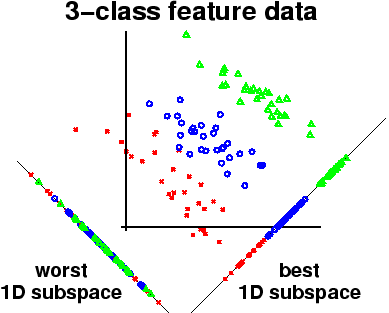
\includegraphics[width=250px]{lda}
  \caption{Linear discriminant analysis on three classes from a two-dimensional space to a one-dimensional subspace.}
  \label{lda}
\end{figure}

We can see in the plot \ref{lda} that the LDA has accomplished its
goal: the within class subspace covariance is obviously smaller than
the one in the original space and the separation between classes is
easily done.

A common approach to project vectors into a better subspace is to
train a projection matrix offline using a training database with a lot
of classes (different speakers). Then, during the speaker verification process, we only
have to project our vectors using our newly learned projection matrix.

\chapter{Spherical Discriminant Analysis}

In this chapter, we will present a dimension reduction technique
called Spherical Discriminant Analysis (SDA). This technique is quite
similar to the LDA, but is using the cosine distance instead of the
euclidean distance.

\newcommand{\argmax}[1]{\smash{\mathop{{\rm argmax}}\limits_{W}}\, #1}
\newcommand{\argmin}[1]{\smash{\mathop{{\rm argmin}}\limits_{W}}\, #1}

\section{Cosine distance}

The cosine distance is a well-used distance which only considers the
direction of a data point and not its norm like the usual euclidean distance.

$$a.b = ||a||.||b||. \cos{\theta}$$
$$\text{cosine similarity} = \cos{\theta} = \frac{a.b}{||a||.||b||}$$
$$\text{cosine distance} = 1 - \cos{\theta} = 1 - \frac{a.b}{||a||.||b||}$$

\begin{figure}[H]
  \centering
  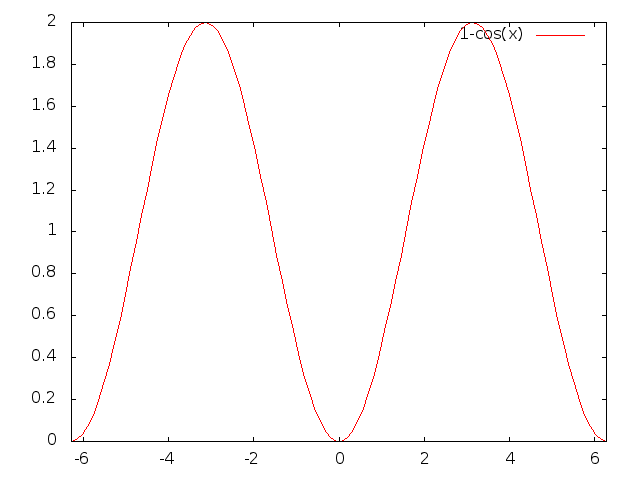
\includegraphics[width=250px]{cosine_distance}
  \caption{Cosine distance plot where $x$ is the angle between two
    vectors.}
  \label{cosine_distance}
\end{figure}

\section{Gradient descent}

The gradient descent is one of the most used optimization method. It's
an iterative method which consists in using the derivative at each
iteration to head towards the local optimum (minimum or maximum).

\begin{figure}[H]
  \centering
  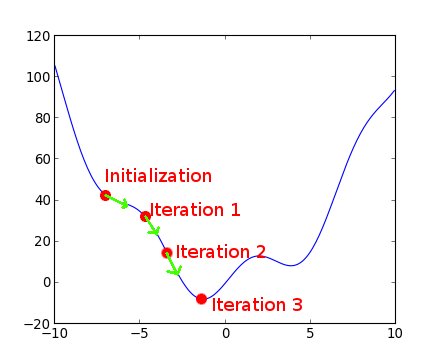
\includegraphics[width=250px]{gradient_descent}
  \caption{Gradient descent with only one parameter. The local minimum found is -10 with parameter -1.}
  \label{gradient_descent}
\end{figure}

\begin{figure}[H]
  \begin{lstlisting}[frame=single]
    while not converge:
        for parameter in parameters:
                parameter = parameter - alpha * derivative_parameter(parameters);
  \end{lstlisting}
  \caption{Gradient-descent algorithm}
  \label{algo_gradient_descent}
\end{figure}

In the algorithm \ref{algo_gradient_descent}, the alpha refers to the
step. If the step is too low, the convergence will be very
slow. However, if the step is too high, the algorithm may not
converged. The big issue in the gradient descent method is to find a
step suitable for the problem.

Fortunately, there are other gradient descent methods which don't
require to choose a step.

\subsection{Resilient backpropagation}

The idea behind the resilient back-propagation (Rprop) is to have
dynamic steps unique to each parameter.
The update rules of these steps are:
\begin{itemize}
\item Speed up: Increase the step when the previous partial derivative and the
  current partial derivative have the same sign;
\item Slow down: Decrease the step otherwise.
\end{itemize}

This method has two advantages:
\begin{itemize}
\item We don't have to choose a step;
\item The convergence may be faster thanks to the speed ups.
\end{itemize}

%BONUS: add pseudocode

\section{Principle}

We have previously seen that we are using a cosine distance between
two low-dimensional vectors to compute a score between two speaker's
utterances. The idea behind the Spherical Discriminant Analysis is
similar to the idea of the Linear Discriminant Analysis: we want to
maximize the distance between two different speakers while minimizing
the distance between two same speakers. The only difference is that we
are using the cosine distance instead of the euclidean distance so
that the scoring, hence the decision, is more accurate.\\ Concretely,
we want to find a projection matrix $W$ from the I-vector space to our
SDA subspace such as:

$$W = \argmin(S_b - S_w)$$
with
$$S_b =
\frac{1}{c(c-1)}\sum_{m=1}^c\sum_{n=1}^c\frac{1}{|D_m||D_n|}\sum_{\substack{x_i
    \in D_m \\ x_j \in D_n}}
\frac{x_i^TWW^Tx_j}{\sqrt{x_i^TWW^Tx_i}\sqrt{x_j^TWW^Tx_j}} (m \neq
n)$$ and
$$S_w = \frac{1}{c}\sum_{i=1}^c\frac{1}{|D_i|^2}\sum_{x_j,x_k \in D_i}
\frac{x_j^TWW^Tx_k}{\sqrt{x_j^TWW^Tx_j}\sqrt{x_k^TWW^Tx_k}}$$
where:
\begin{itemize}
  \item $c$: number of speakers;
  \item $D_i$: I-vectors of the speaker $i$;
  \item $|D_i|$: number of I-vectors of the speaker $i$.
\end{itemize}

$S_b$ is the between-class cosine similarity of the projected
space. It is simply the average cosine similarity (opposite of the
cosine distance) between the data points of different classes. In this
situation it is the average cosine similarity between the speech
utterances of different speakers.

Similarly, $S_w$ is the within-class cosine similarity of the
projected space. It is the average cosine similarity between the
speech utterances of same speakers.\\
By finding a projection matrix $W$ minimizing the between-class cosine
similarity while maximizing the within-class cosine similarity we find
a subspace suitable for cosine distance scoring.

\section{Algorithm}

In order to find this matrix, we have to find the derivative of $S_b -
S_w$ in order to apply a gradient descent method. %CORRECT: phrase bizarre

Let $F(W) = S_b - S_w$, then the derivative is defined as below:
$$\frac{\partial{F(W)}}{\partial{W}} =
2\sum_{i\neq{}j}\left[\frac{f_{ij}x_ix_i^TW}{f_i^3f_j} +
  \frac{f_{ij}x_jx_j^TW}{f_j^3f_i} - \frac{x_ix_j^TW + x_jx_i^TW}{f_if_j}\right]s_{ij}$$
Where:
\begin{itemize}
\item $f_{ij} = x_i^TWW^Tx_j$
\item $f_i = \sqrt{x_i^TWW^Tx_i}$
\item $s_{ij} = \frac{1}{c|D_i||D_i|}$ if $x_i$ and $x_j$ belong to the same class
\item $s_{ij} = -\frac{1}{c(c-1)|D_i||D_j|}$ otherwise
\end{itemize}

We now only have to find the projection matrix $W$ which minimize
$F(W)$ using the previously seen gradient descent method with the
derivative $\frac{\partial{F(W)}}{\partial{W}}$.
%BONUS: \subsection{Demonstration of the derivative}


\subsection{Example}

Let us have a small experiment to understand and observe the
convergence of this algorithm.  For this experiment we only have three
different speakers and the subspace dimension is chosen to be two in
order to be able to plot the projected data.

Once the projection matrix $W$ is computed, the projection is done by:
$$y_i = \frac{W^Tx_i}{||W^Tx_i||}$$ The normalization term is not
mandatory for we use the cosine distance (which normalizes) but it
gives a better idea on the plot of the cosine distance.

\begin{figure}[H]
  \centering
  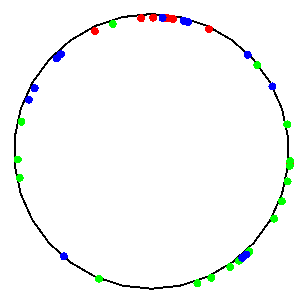
\includegraphics[width=150px]{draw0}
  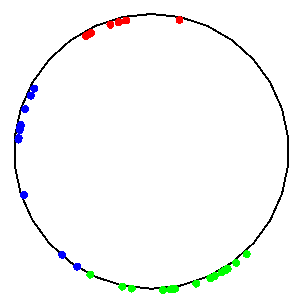
\includegraphics[width=150px]{draw1}
  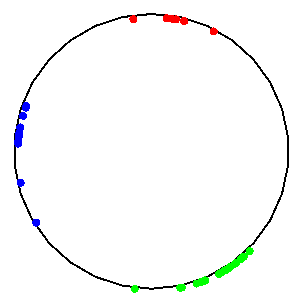
\includegraphics[width=150px]{draw2}
  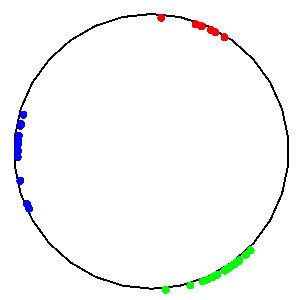
\includegraphics[width=150px]{draw3}
  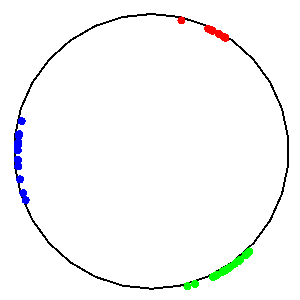
\includegraphics[width=150px]{draw4}
  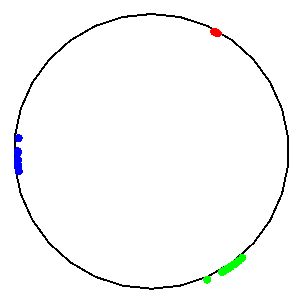
\includegraphics[width=150px]{draw8}
  \caption{Projected data plots by the randomly initialized matrix and
    by the matrix after one, two, three, four and eight iterations. A
    data point is a speech utterance and a speaker is represented by a
    color.}
  \label{draws}
\end{figure}


The projected data is on a circle due to the data normalization.  We can
observe in the figure \ref{draws} that, over the iterations, the
average distance between the different speakers increased while the
average distance between the same speakers decreased.

\section{Implementation}
In this part, I will discuss the implementation specifications, issues
and solutions found.

\subsection{Specifications}

The implementation was made in C++ using the Blas library for matrix
computations.  However, due to the numerous required calls to Blas and
its heavy syntax, I decided to do an overlay matrix class which will
dispatch calls to Blas. This allowed me to have a Matlab-like syntax.

\lstset{language=c++}
\begin{figure}[H]
  \begin{lstlisting}[frame=single, caption=Source]
    Matrix mat(3,3);
    Matrix mat2("[1 2 3; 4 5 6; 7 8 9]");

    mat.zero();
    mat[0][0] = 42.0;
    mat = mat * mat2 - mat2 + mat * 2.0;

    std::cout << mat << std::endl;
    std::cout << mat[0] << std::endl;
  \end{lstlisting}

  \begin{lstlisting}[frame=single, caption=Output]
    3 3
    125 82 123
    -4 -5 -6
    -7 -8 -9

    1 3
    125 82 123
  \end{lstlisting}
  \caption{Usage of matrix class}
  \label{algo_matrix}
\end{figure}

\subsection{Issues}

A big issue in this projection method is the derivative computation
because it's computationally expensive.
Let's have a quick look at the complexity of the derivative computation.

$$\frac{\partial{F(W)}}{\partial{W}} =
2\sum_{i\neq{}j}\left[\frac{f_{ij}x_ix_i^TW}{f_i^3f_j} +
  \frac{f_{ij}x_jx_j^TW}{f_j^3f_i} - \frac{x_ix_j^TW + x_jx_i^TW}{f_if_j}\right]s_{ij}$$

$$\frac{\partial{F(W)}}{\partial{W}} =
2\sum_{j}\sum_{i\neq{}j}\left[\frac{f_{ij}x_ix_i^TW}{f_i^3f_j} +
  \frac{f_{ij}x_jx_j^TW}{f_j^3f_i} - \frac{x_ix_j^TW + x_jx_i^TW}{f_if_j}\right]s_{ij}$$

Let $n$ be the total number of data points (speech utterances), $d$ be
the dimension of the data and $d'$ the dimension of the projected
data.

Then, the complexity is equal to:
$$\circ{(n^2.(d^2.d'+d.d'+d'^2))} = \circ{(n^2.(d^2.d'+d'^2))} = \circ{(n^2d^2d'+n^2d'^2)}$$
In our application we have:
\begin{itemize}
  \item $n = 30000$
  \item $d = 600$
  \item $d' = 250$
\end{itemize}

Given that we have to do this computation at each iteration, we see
that we have to rethink this equation in order to get rid of most of
the computation of complexity $n^2$.

$$\frac{\partial{F(W)}}{\partial{W}} =
2\sum_{j}\sum_{i\neq{}j}\left[\frac{x_i^TWW^Tx_jx_ix_i^T}{f_i^3f_j} +
  \frac{x_i^TWW^Tx_jx_jx_j^T}{f_j^3f_i} - \frac{x_ix_j^T + x_jx_i^T}{f_if_j}\right]Ws_{ij}$$

$$\frac{\partial{F(W)}}{\partial{W}} =
2\sum_{j}\sum_{i\neq{}j}\left[2\frac{x_i^TWW^Tx_jx_ix_i^T}{f_i^3f_j}
   - \frac{x_ix_j^T + x_jx_i^T}{f_if_j}\right]Ws_{ij}$$

$$\frac{\partial{F(W)}}{\partial{W}} =
2\sum_{j}\sum_{i\neq{}j}\left[2\frac{x_ix_i^Tx_i^TWW^Tx_j}{f_i^3f_j}
   - \frac{x_ix_j^T + x_jx_i^T}{f_if_j}\right]Ws_{ij}$$

$$\frac{\partial{F(W)}}{\partial{W}} =
2\sum_{i}\sum_{j\neq{}i}\left[2\frac{x_ix_i^Tx_i^TWW^Tx_j}{f_i^3f_j}
   - \frac{x_ix_j^T}{f_if_j} - \frac{x_jx_i^T}{f_if_j}\right]Ws_{ij}$$

$$\frac{\partial{F(W)}}{\partial{W}} =
2\sum_{i}\left[2\frac{x_ix_i^Tx_i^TWW^T}{f_i^3}\sum_{j\neq{}i}\frac{x_js_{ij}}{f_j}
  - \sum_{j\neq{}i}\left[\frac{x_ix_j^Ts_{ij}}{f_if_j} - \frac{x_jx_i^Ts_{ij}}{f_if_j}\right]\right]W$$

$$\frac{\partial{F(W)}}{\partial{W}} =
2\sum_{i}\left[2\frac{x_ix_i^Tx_i^TWW^T}{f_i^3}\sum_{j\neq{}i}\frac{x_js_{ij}}{f_j}
  - A_i - A_i^T\right]W$$

$$\text{with: } A_i = \frac{x_i}{f_i}\sum_{j\neq{}i}\frac{x_js_{ij}}{f_j}$$
New complexity: $$\circ{(n^2.d+n.d^2.d')}$$

\chapter{Experiments and results}

This chapter describes the obtained results given by the experiments
realized to test our dimension reduction method. First, the whole step
of parametrization, the used tools and the used corpus to perform
the NIST 2012 Speaker Recognition (SRE) campaign are described. Then, the results are
presented and compared to the results obtained from the Probabilistic
Linear Discriminant Analysis (PLDA).

\section{Experiments}

This section describes the experiments realized to compare the
dimension reduction methods. These experiments are performed on the
trials of the NIST 2012 SRE campaign which consists in training 2204
speakers and performing 576672196 tests. %CORRECT: Faux chiffres.

\subsection{Features extraction}

The features extraction is processed by HTK. First, this one sampled
the speech signal every 10ms on a 25ms sliding window. From this
window, the energy and 19 Mel-Frequency Cepstral Coefficients (MFCCs)
are extracted.  Then, the first and second order deltas are
computed. A 60-dimensional cepstral vector is obtained by taking the
19 MFCCs, the energy, the 20 first order deltas and the 20 second
order deltas.\\\\ These coefficients are known to match the variation
of the human ear's most important frequency bandwidths. In order to
extract the phonetically important traits of speech, the Mel scale
uses filters based on linear scales as well as logarithm scales. MFCCs
partially absorb variations caused by the physical condition of the
speakers vocal cord.

\subsection{Voice activity detection/Speaker diarization}

To get rid of the noise/silence segments, we use an energy-based voice
activity detection method described in the paper of \cite{CRIM}.  This
method reside in learning two generative models (Gaussian Mixture
Model): one for speech and one for noise and silence. This enable us
to keep the segment if the segment is likelier to belong to the speech
model than the noise model.

\subsection{Modeling}

We build probabilistic speaker models which are large GMMs of 2048
components with diagonal covariance matrices by a Maximum A Posteriori
(MAP) adaptation from the Universal Background Model (UBM) which is a
large GMM representing every speaker.  This UBM is trained offline
thanks to the Expectation Maximization (EM) algorithm.  From this
newly built speaker GMM, we concatenate the mean of every component to
obtain a super-vector of dimension 122880. Then, we can obtain a
low-dimensional vector called i-vector.

\subsection{Dimension reduction}

This part is the only variable part. We will use the Probabilistic
Linear Discriminant Analysis (PLDA) as a reference and try the
Spherical Discriminant Analysis (SDA) described in this paper.

\subsection{Scoring}

The scoring is just the cosine similarity between two projected i-vectors.
In practice, we are doing the projection and the scoring at the same time:
Let $y_i$ the projected i-vector, $x_i$ the i-vector and $P$ the projection matrix.\\
Then the score is defined as follow:
$$\text{score} = \frac{y_i^Ty_j}{|y_i||y_j|}$$
with
$$y_i = P^Tx_i$$
$$\text{score} = \frac{x_i^TPP^Tx_j}{|x_i^TP||x_j^TP|}$$ We now have a
scalar that we just have to threshold to make a decision.  The
threshold represents the sensibility of the system: a low threshold
will induce to accept easily a speaker while a high threshold will
induce a lot of rejections.

The system has to be calibrated to find a trade-off between
acceptations and rejections. That is why we introduce the Decision
Error Trade-off (DET).

\section{Results}

The results are presented using Decision Error Trade-off (DET)
curves. These enable to compare different speaker verification
systems. The performances are represented by plotting the false-alarm
probability $P_{FalseAlarm}$ as a function of the miss error
probability $P_{Miss}$. The probability $P_{FalseAlarm}$ corresponds
to the probability to reject a target speaker while the probability
$P_{Miss}$ corresponds to the probability to accept a non-target
speaker (or impostor). Unfortunately, it is generally not possible to
minimize $P_{FalseAlarm}$ and $P_{Miss}$ together. Thus, the DET
curves underline the trade-off between the miss errors and the
false-alarm errors. Given a false-alarm error rate, we can infer the
corresponding miss error rate and vice-versa. So a system is better
than another if its DET curve is closer to the origin point than the
other DET curve.  Another criterion to compare speaker verification
systems is to study specific points of the DET curves. Generally,
systems are compared by studying the point where the two probabilities
$P_{FalseAlarm}$ and $P_{Miss}$ are equal. This point is characterized
by the equal probability known as the Equal Error Rate (EER). However,
in the speaker verification task, it is preferable to reject
clients than to accept impostors to intrude in the system. That is
given by studying the point which minimized a Decision Cost Function
(DCF). The DCF is a function which assigns a cost for each kind of
errors. Actually, the DCF promotes the false-alarm errors and
penalizes the miss errors. Thus the DCF is defined as a weighted sum
of miss and false-alarm error probabilities given by

$$C_{CDF} = C_{Miss}.P_{Miss}.P_{Target} + C_{FalseAlarm}.P_{FalseAlarm}.(1 - P_{Target})$$

where $C_{Miss}$ and $C_{FalseAlarm}$ are respectively the associated
costs to a miss and a false-alarm error. The $P_{Target}$ is the
probability to have a true access.

\begin{figure}[H]
  \centering
  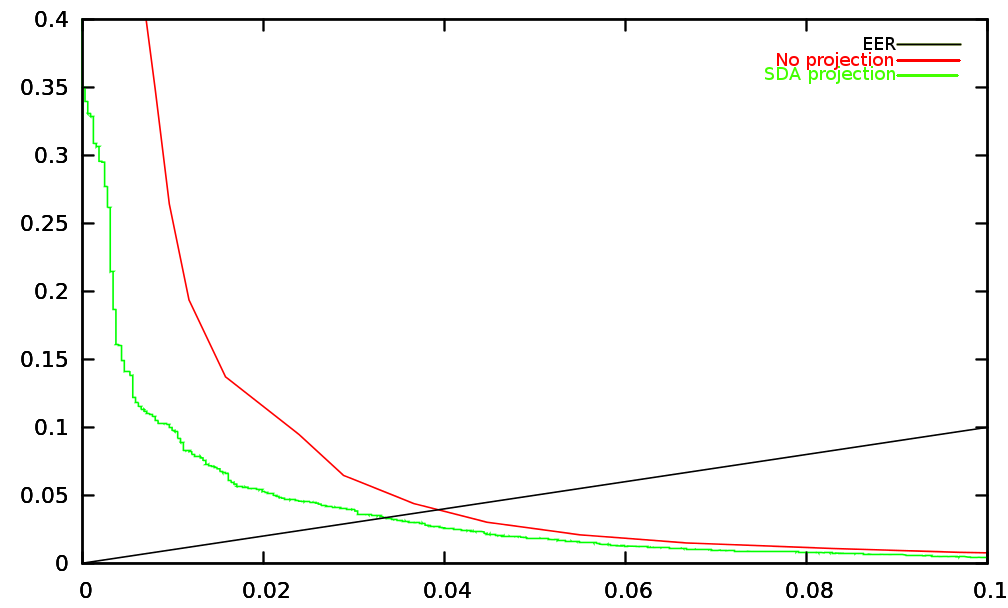
\includegraphics[width=450px]{det_curves}
  \caption{DET curves.}
  \label{lda}
\end{figure}

\section{Discuss}
%TODO: Previous work, Related work, future work

\chapter*{Conclusion}
%TODO: Quelques paragraphes. Une conclusion qui résume clairement le contenu
%de votre rédaction, dans le même ordre que le contenu présenté était
%détaillé. La conclusion doit ensuite mettre l’accent sur les
%principaux intérêts / fonctionnalités de ce que vous avez présenté et
%mettre en avant votre travail.  Ne pas se contenter de faire une
%resucée du résumé. D’ailleurs, ce n’est pas une «synthèse», c’est une
%«conclusion». En d’autres termes, ne pas s’arrêter à un résumé de
%l’article, mais finir en ouvrant le débat : quelles pistes restent
%encore à explorer, quels nouvelles questions ou problèmes se posent,
%quels autres sujets semblent liés etc.

\chapter*{Acknowledgement}

Thanks to my supervisor Reda Dehak for his explanations, to Laurent
Senta, Pierre Parutto for their proofreading and to all the LRDE for
their support.

\bibliography{final_report} \nocite{*}
\end{document}
